\begin{figure}[ht!]
\centering
\begin{minipage}{.5\textwidth}
  \centering
  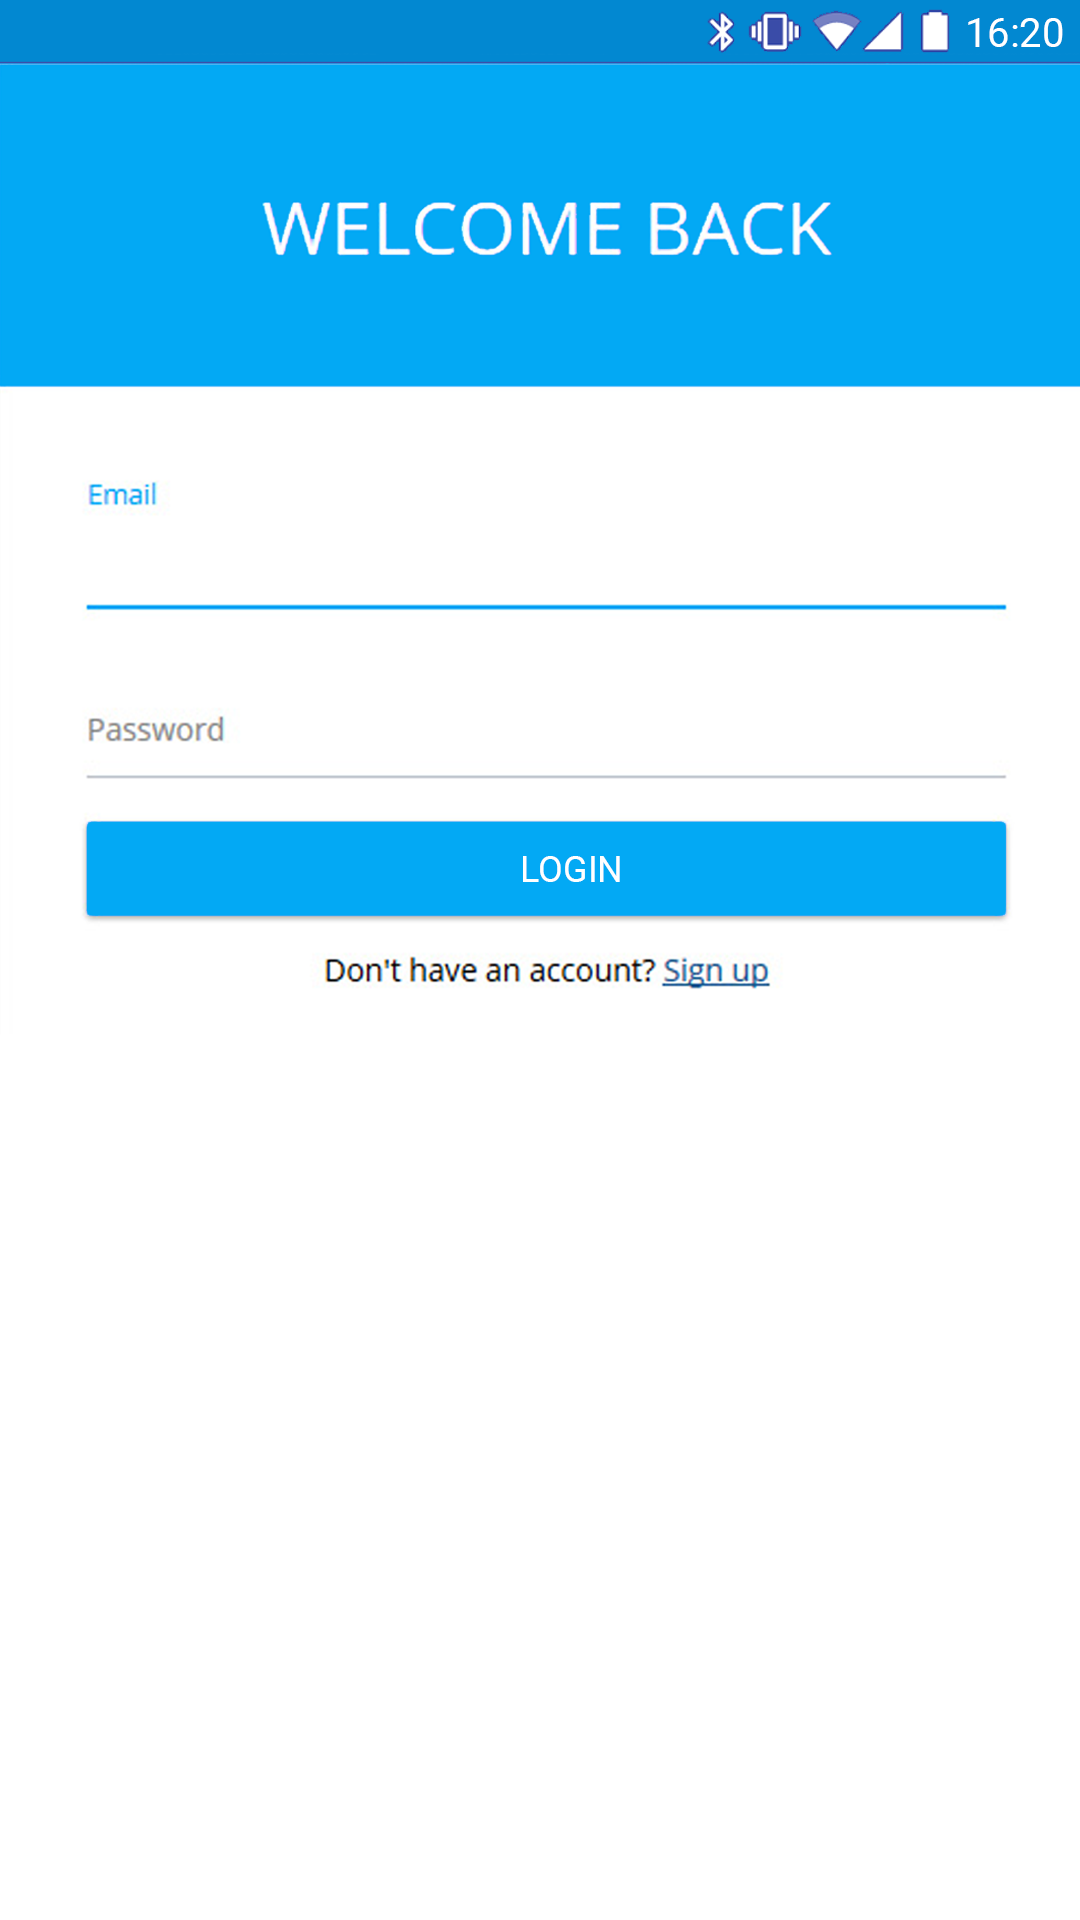
\includegraphics[width=0.9\linewidth]{manual/Login.png}
  \caption{\label{fig:vitals}The login screen}
Main screen to log into ReVA. 
   1. The login button to be clicked once all necessary information has been filled out. 
   2. The registration link that may be tapped in case users do not have an existing login. 
   3. User password input section. (Needed for verification and validation before ReVA login). 
   4. User email address input section. (Used as a username to identify users). 
\end{minipage}%
\begin{minipage}{.5\textwidth}
  \centering
  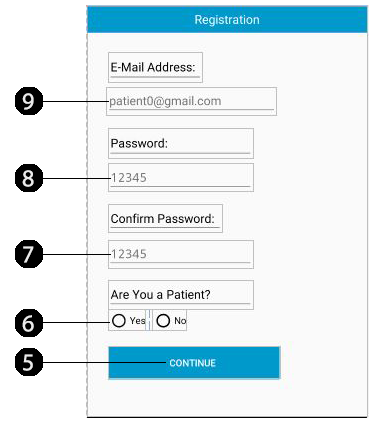
\includegraphics[width=0.9\linewidth]{manual/registration1.png}
  \caption{\label{fig:statistic}The registration screen 1}
\end{minipage}
\end{figure}
First page of registration (used by both subscribers and patients). 
  5. The continue button to proceed with the registration. 
  6. Yes/No radio button input to decide whether the user is a patient or subscriber. 
  7. Password confirmation input. 
  8. Password input for password that will be used for user login. 
  9. Email input for the email that will be used for user login. 

\begin{figure}[ht!]
\centering
\begin{minipage}{.5\textwidth}
  \centering
  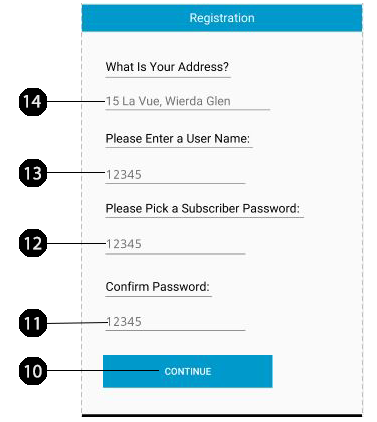
\includegraphics[width=0.9\linewidth]{manual/registration2.png}
  \caption{\label{fig:vitals}The registration screen 2}
Second page of user registration (meant only for patients). 
  10. The continue button for patients to proceed with the registration process. 
  11. Confirm password input for subscriber password. 
  12. Subscriber password input. (Will be used to verify and validate users wishing to subscribe to current patient). 
  13. Username input. (Will be used to identify patients). 
  14. Address input. (Stored in case of serious emergencies). 

\end{minipage}%
\begin{minipage}{.5\textwidth}
  \centering
  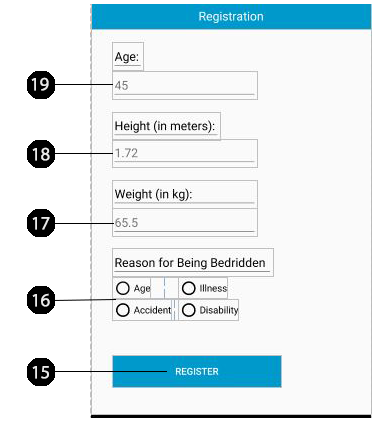
\includegraphics[width=0.9\linewidth]{manual/registration3.png}
  \caption{\label{fig:statistic}The registration screen 3}
\end{minipage}
\end{figure}
Third page of user registration (meant only for patients). 
  15. Register button. (Registers patient that has filled in all necessary information). 
  16. Bedridden reason radio input section. (Used to store the reason for patient being bedridden). 
  17. Weight input. (Used for measuring patient vitals more accurately). 
  18. Height input. (Used for measuring patient vitals more accurately). 
  19. Age input. (Used for measuring patient vitals more accurately). 

\begin{figure}[ht!]
\centering
\begin{minipage}{.5\textwidth}
  \centering
  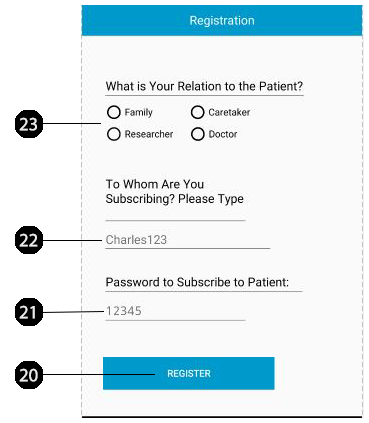
\includegraphics[width=0.9\linewidth]{manual/registration4.png}
  \caption{\label{fig:vitals}The registration screen 4}

\end{minipage}%
\begin{minipage}{.5\textwidth}
  \centering
  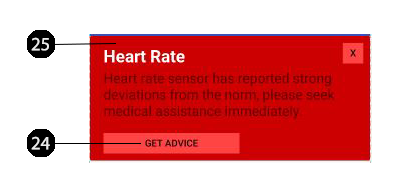
\includegraphics[width=0.9\linewidth]{manual/notification.png}
  \caption{\label{fig:statistic}The notifications screen}
\end{minipage}
\end{figure}

\begin{figure}[ht!]
\centering
\begin{minipage}{.5\textwidth}
  \centering
  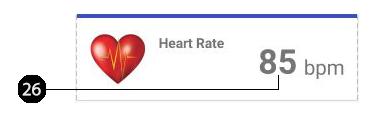
\includegraphics[width=0.9\linewidth]{manual/real-time.png}
  \caption{\label{fig:vitals}The real-time data screen 4}

\end{minipage}%
\begin{minipage}{.5\textwidth}
  \centering
  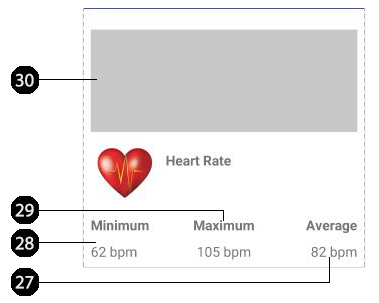
\includegraphics[width=0.9\linewidth]{manual/statistics.png}
  \caption{\label{fig:statistic}The statistics screen}
\end{minipage}
\end{figure}
